\newcommand{\decktitle}{Kommandozeile}

%%%%%%%%%%%%%%%%%%%%%%%%%%%%%%%%%%%%%%%%%%%%%%%%%
%
% DOCUMENT
%
%%%%%%%%%%%%%%%%%%%%%%%%%%%%%%%%%%%%%%%%%%%%%%%%%

\begin{frame}
    \subtitle{\decktitle}
    \titlepage
\end{frame}


\begin{frame}
    \frametitle{\textbf{Outline:}}
    \tableofcontents
\end{frame}

		
		   
\section{Kommandozeile}

    \begin{frame}{Was ist die Kommandozeile?}
    
        \begin{itemize}
            \item Annähernd jedes Betriebssystem besitzt eine Kommandozeile
            \item Eine Kommandozeile nimmt Befehle vom Nutzer, die dieser bspw. eintippen kann, entgegen und führt diese aus
            \item Zu Beginn des Computerzeitalters war dies oftmals die einzige Möglichkeit, Befehle / Programme auszuführen, da graphische Benutzeroberflächen (GUIs) erst später verbreitet waren
            \item Auch heute wird die Kommandozeile noch häufig verwendet (insbesondere von Entwicklern), da hierdurch Befehle sehr schnell ausgeführt werden können und der Nutzer nicht erst in der GUI danach suchen muss
            \item Die Kommandozeile besitzt verschiedene Namen: \textit{Eingabeaufforderung}, \textit{Befehlszeile}, \textit{Terminal}, \textit{CLI (command-line interface)}, \textit{command prompt}, ...
        \end{itemize}
    \end{frame}
    
    \begin{frame}{Wofür benötigen wir die Kommandozeile?}
        In der Programmierung ist die Kommandozeile unabdingbar. Oftmals sind Befehle notwendig, die über die GUI nur sehr schwer (oder überhaupt nicht) ausgeführt werden können, außerdem trägt die Verwendung der Kommandozeile zum Grundverständnis verschiedenster Operationen bei. \\~\
        
        Eine Auswahl der wichtigsten Operationen werden im Folgenden vorgestellt und sollen im Anschluss auch angewendet werden können.
    \end{frame}
    
    
    \begin{frame}{Öffnen der Kommandozeile (Windows 10)}
        In Windows wird die Kommandozeile im Deutschen "\textit{Eingabeaufforderung}" genannt. Diese kann auf unterschiedliche Arten geöffnet werden:
        
        \begin{itemize}
            \item Start \textrightarrow Windows-System \textrightarrow Eingabeaufforderung
            \item \texttt{WIN}-Taste + \texttt{R} \textrightarrow  \texttt{cmd} eingeben \textrightarrow Bestätigen
        \end{itemize}
        
        
        \begin{figure}
            \centering
            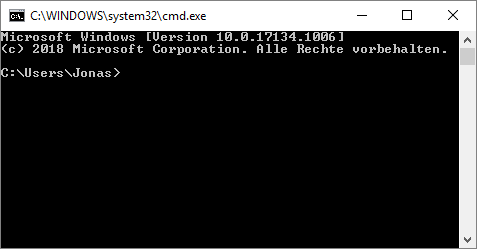
\includegraphics[width=0.8\linewidth,height=0.5\textheight,keepaspectratio]{chapters/05_command_line/figures/cmd_win.png}
            \caption{Die Windows-Eingabeaufforderung}
        \end{figure}
        
    \end{frame}
    
    \begin{frame}{Öffnen der Kommandozeile (macOS)}
        In macOS wird die Kommandozeile "\textit{Terminal}" genannt. Diese kann folgendermaßen geöffnet werden:
        
        \begin{itemize}
            \item Finder \textrightarrow Programme \textrightarrow Dienstprogramme \textrightarrow Terminal
        \end{itemize}
        
        \begin{figure}
            \centering
            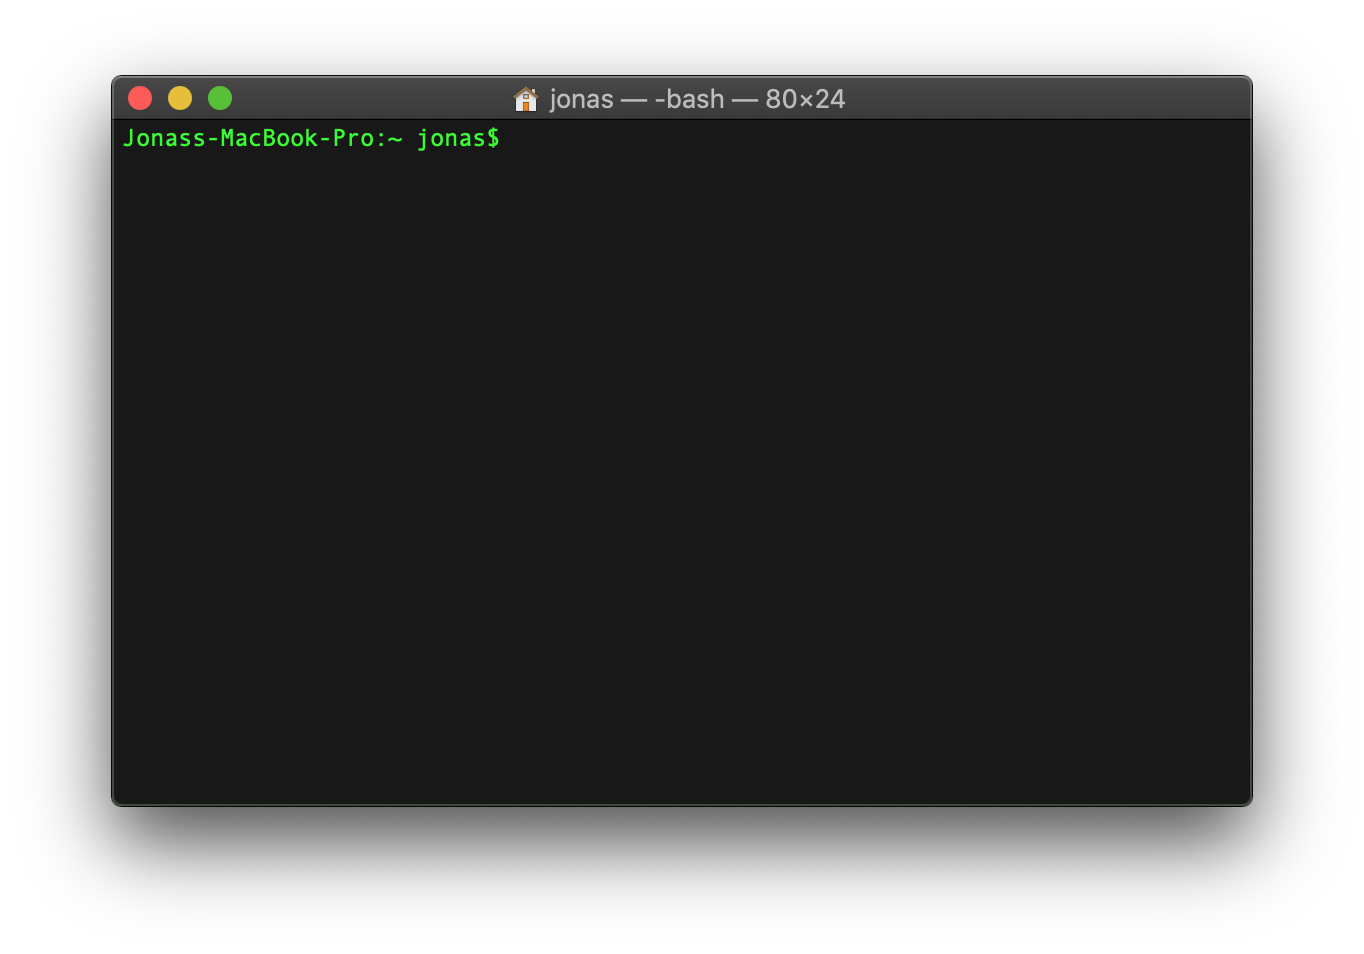
\includegraphics[width=0.8\linewidth,height=0.5\textheight,keepaspectratio]{chapters/05_command_line/figures/cmd_mac.png}
            \caption{Die macOS-Eingabeaufforderung}
        \end{figure}
    \end{frame}

    \begin{frame}{Verwenden der Kommandozeile}
        Mithilfe der Kommandozeile ist es möglich, ebenso wie mit dem Windows Dateiexplorer bzw. dem Finder auf macOS, durch das Dateisystem zu navigieren.
        Die Kommandozeile zeigt stets an, in welchem Ordner sich der Nutzer aktuell befindet. \\~\
        
        Wird also angezeigt \code{C:\textbackslash{}Users\textbackslash{}Jonas} bedeutet das, dass sich der Nutzer aktuell in seinem Nutzerverzeichnis befindet. Bei macOS enthält die Anzeige (z.B. \code{Jonas-MacBook-Pro:$\sim$ jonas}) standardmäßig noch zusätzliche Informationen: Der erste Teil bezieht sich auf den Computernamen (\code{Jonas-MacBook-Pro}), nach dem Doppelpunkt folgt der aktuelle Ordner (\code{$\sim$}), sowie der aktuell angemeldete Nutzer (\code{jonas}).
    \end{frame}
    
    \begin{frame}{Verwenden der Kommandozeile}
        \begin{alertblock}{Achtung}
            Bei Windows werden Dateipfade standardmäßig mit Backslash (\code{\textbackslash{}}) geschrieben. Auf unixoiden Systemen wie macOS oder Linux wird standardmäßig ein Forwardslash (\code{/}) verwendet.
        \end{alertblock}
    \end{frame}
    
    \begin{frame}{Verwenden der Kommandozeile - Dateisystem}
        In der Regel sind die Dateisysteme bei allen Betriebssystemen hierarchisch aufgebaut. \\~\
        
        \begin{itemize}
            \item \textbf{Windows:} Bei Windows bekommt jede Speichereinheit (z.B. Festplatte) einen Buchstaben zugewiesen. Die primäre Speichereinheit trägt i.d.R. den Namen \code{C}. Diese Speicherinhalt beinhaltet dann verschiedene Dateien und Verzeichnisse, welche wiederum Dateien und Verzeichnisse enthalten können. Ein Unterverzeichnis von C kann z.B. der Ordner \texttt{Benutzer} (oder \texttt{Users}) sein, in dem alle benutzerspezifischen Informationen abgelegt sind. Ein weiterer Ordner ist bspw. \texttt{Programme}, der alle notwendigen Dateien der installierten Programme beinhaltet.
        \end{itemize}
    \end{frame}
    
    \begin{frame}{Verwenden der Kommandozeile - Dateisystem}
       
        \begin{itemize}
            \item \textbf{macOS:} In unixoiden Betriebssystem ist das Dateisystem ebenfalls hierarchisch, jedoch etwas anders aufgebaut. Während es bei Windows mehrere \textit{Roots} geben kann (eine für jede Speichereinheit), gibt es bei unixoiden System stets lediglich eine \textit{Root}, nämlich \code{/}. Hierunter befinden sich ebenfalls hierarchisch die verschiedenen Ordner und Dateien. In Abb. \ref{fig:file_system} wird der Aufbau der Dateisysteme exemplarisch gezeigt.
        \end{itemize}
    \end{frame}
    
     \begin{frame}{Verwenden der Kommandozeile - Dateisystem}
       
       \begin{figure}
            \centering
            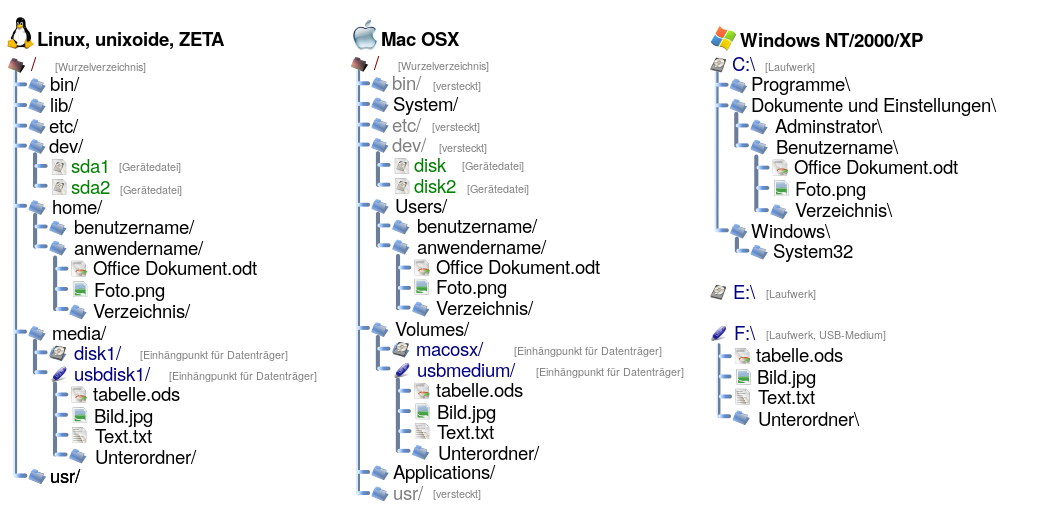
\includegraphics[width=\linewidth,height=0.7\textheight,keepaspectratio]{chapters/05_command_line/figures/Filesystem.png}
            \caption{Vergleich der Verzeichnisstruktur verschiedener Betriebssysteme \cite{filesystems}}
            \label{fig:file_system}
        \end{figure}
    \end{frame}
    
     \begin{frame}{Verwenden der Kommandozeile - Navigieren}
        Wie mit dem Dateiexplorer auch kann mithilfe der Kommandozeile durch die Verzeichnisse navigiert werden. Der Befehl hierfür lautet \code{cd} ("change directory"). \\~\
        
        Es kann entweder ein \textbf{absoluter} Pfad, der das Verzeichnis ausgehend von der Root beschreibt, oder ein \textbf{relativer} Pfad, der das Verzeichnis ausgehend vom aktuellen Verzeichnis beschreibt, angegeben werden. \\~\
        
        Bei Windows beginnt ein absoluter Pfad immer mit \code{C:\textbackslash{}} bzw. \code{\textbackslash{}}. Bei macOS beginnt ein absoluter Pfad immer mit \code{/}.
     \end{frame}
     
     
     \begin{frame}{Verwenden der Kommandozeile - Navigieren}
        
        \begin{itemize}
            \item \textbf{Betreten eines nächst-tieferen Verzeichnisses:} Angenommen das Verzeichnis, in dem sich der Nutzer gerade befindet, beinhaltet ein Verzeichnis mit dem Namen \textit{Programming}. Nun kann in dieses Verzeichnis gewechselt werden, in dem der Nutzer folgenden Befehl eingibt: \\~\
            
            \code{cd Programming}
            
            Dies stellt einen relativen Pfad dar, da ausgehend vom aktuellen Verzeichnis in das "tiefere" Verzeichnis "Programming" gewechselt wird. Folgende absolute Pfadangabe wäre äquivalent: \\~\
            
            \code{cd C:\textbackslash{}Users\textbackslash{}Jonas\textbackslash{}Programming} (Windows) bzw. \code{cd /Users/Jonas/Programming} (macOS)
            
        \end{itemize}
        
     
     \end{frame}
     
      \begin{frame}{Verwenden der Kommandozeile - Navigieren}
        
        \begin{itemize}
         
            \item \textbf{Betreten des übergeordneten Verzeichnisses:} Der Nutzer kann in das übergeordnete Verzeichnis wechseln, indem er folgendes eingibt: \\~\
            
            \code{cd ..}
            
            \begin{block}{Hinweis}
                \code{..} steht üblicherweise als Abkürzung für das übergeordnete Verzeichnis, während \code{.} für das aktuelle Verzeichnis steht
            \end{block}
        \end{itemize}
    
     \end{frame}
     
      \begin{frame}{Verwenden der Kommandozeile - Navigieren}
        
        \begin{itemize}
         
            \item \textbf{Betreten des Nutzerverzeichnisses:}
                
                \begin{itemize}
                    \item \textbf{macOS:} Unter macOS gibt es eine Kurzschreibweise um in das Nutzerverzeichnis (Home-Verzeichnis) zu wechseln. Auf unixoiden System steht das Symbol \code{$\sim$} i.d.R. für das Nutzerverzeichnis, also reicht der folgende Befehl aus: \\~\
                
                    \code{cd $\sim$} bzw. \code{cd} (äquivalent zu \code{cd /Users/Jonas/}) \\~\
                    
                    \item \textbf{Windows:} Bei Windows existiert eine solche Kurzform nicht, falls aber die Umgebungsvariable \code{HOMEPATH} gesetzt ist, kann dieser Befehl genutzt werden: \\~\
                
                \code{cd \%HOMEPATH\%}
                \end{itemize}
                
        \end{itemize}
    \end{frame}
    
    \begin{frame}{Verwenden der Kommandozeile - Anzeigen des aktuellen Verzeichnisses}
        Um den kompletten (absoluten) Pfad des Verzeichnisses, in dem sich der Nutzer derzeit befindet, anzuzeigen, gibt es betriebssystemspezifische Befehle:
        
        \begin{itemize}
            \item \textbf{Windows:} \code{cd}
            \item \textbf{macOS:} \code{pwd} (print working directory)
        \end{itemize}
    \end{frame}
    
    \begin{frame}{Verwenden der Kommandozeile - Anzeigen von Verzeichnisinhalten}
        Um die Inhalte von Verzeichnissen anzuzeigen, also alle im derzeitigen Verzeichnis enthaltenen Dateien und Ordner, gibt es für Windows und macOS verschiedene Befehle:
        
        \begin{itemize}
            \item \textbf{Windows:} \code{dir} (directory)
            \item \textbf{macOS:} \code{ls} (list) (bzw. \code{ls -l}, um die Inhalte in einer Liste mit Details anzuzeigen)
        \end{itemize}
    \end{frame}
    
    
     \begin{frame}{Verwenden der Kommandozeile - Anlegen von Verzeichnissen}
        
        Mithilfe der Kommandozeile können auch Verzeichnisse angelegt werden, ebenso wie im Datei-Explorer ein neuer Ordner angelegt werden kann.\\~\
        
        Hierfür existiert der \code{mkdir}-Befehl. Dieser Benötigt jedoch noch ein zusätzliches \textit{Argument}, mit dem der Name des Verzeichnisses mit angegeben werden kann, also z.B. \\~\
        
        \code{mkdir Programming} \\~\
        
        Hierdurch wird im aktuellen Verzeichnis ein Ordner mit dem Namen "Programming" erzeugt.
    \end{frame}
    
    \begin{frame}{Verwenden der Kommandozeile - Löschen von Verzeichnissen}
        
        Auch ein Löschen von Verzeichnissen und Dateien ist möglich.\\~\
        
        \begin{alertblock}{Achtung}
            Durch das Löschen von Verzeichnissen und Dateien können Informationen unwiderruflich verloren gehen. Es muss also sichergestellt werden, dass lediglich Elemente gelöscht werden, die gelöscht werden sollen.
        \end{alertblock}
        
        \begin{itemize}
            \item \textbf{Windows:} 
                \begin{itemize}
                    \item \textbf{Löschen einer Datei:} \code{del <Dateiname>}
                    \item \textbf{Löschen eines Verzeichnisses:} \code{rmdir /S /Q <Verzeichnisname>}
                \end{itemize}
            \item \textbf{macOS:}
                \begin{itemize}
                    \item \textbf{Löschen einer Datei:} \code{rm <Dateiname>}
                    \item \textbf{Löschen eines Verzeichnisses:} \code{rm -rf <Verzeichnisname>}
                \end{itemize}
        \end{itemize}
        
    \end{frame}
    
    
    \begin{frame}{Verwenden der Kommandozeile - Kopieren von Dateien}
        
        Mithilfe der Kommandozeile können Dateien ebenso wie über den Explorer in andere Verzeichnisse kopiert werden. \\~\
        
        Hierfür existiert der \code{copy} (Windows) bzw. \code{cp} (macOS) Befehl. Dieser Befehl besitzt zwei Argumente: Als erstes muss die Datei angegeben werden, die kopiert werden soll, als zweites muss der Zielpfad spezifiziert werden, z.B.: \\~\
        
        \code{copy main.py ..\textbackslash{}} bzw. \code{cp main.py ../}\\~\
        
        Mithilfe dieses Befehls wird die Datei \code{main.py} aus dem aktuellen Verzeichnis in das übergeordnete Verzeichnis (\code{../}) kopiert.
        
    \end{frame}
    
    \begin{frame}{Verwenden der Kommandozeile - Verschieben von Dateien}
        
        Mithilfe der Kommandozeile können Dateien ebenso wie über den Explorer in andere Verzeichnisse verschoben werden. \\~\
        
        Hierfür existiert der \code{move} (Windows) bzw. \code{mv} (macOS) Befehl. Dieser Befehl besitzt zwei Argumente: Als erstes muss die Datei angegeben werden, die verschoben werden soll, als zweites muss der Zielpfad spezifiziert werden, z.B.: \\~\
        
        \code{move main.py ..\textbackslash{}} bzw. \code{mv main.py ../}\\~\
        
        Mithilfe dieses Befehls wird die Datei \code{main.py} aus dem aktuellen Verzeichnis in das übergeordnete Verzeichnis (\code{../}) verschoben.
        
    \end{frame}
    
\begin{frame}{Verwenden der Kommandozeile - Tipps}
    
    \begin{block}{Ergänzung von Befehlen}
      Mithilfe der Tabulator-Taste können gewisse Befehle und Dateinamen ergänzt werden, wenn die Anfangsbuchstaben eingegeben wurden. \\~\
      
      Beispiel: Es existiert eine Datei namens \code{main.py} im aktuellen Verzeichnis. Wird nun \code{copy ma} eingegeben und anschließend die Tabulator-Taste gedrückt, wird der Dateiname automatisch ergänzt.
    \end{block}
    
    \begin{block}{Durchsuchen des Befehlsverlaufs}
      Mithilfe der Pfeil-Tasten (\textuparrow / \textdownarrow) können die letzten Befehle durchgegangen und erneut ausgeführt werden.
      
    \end{block}
\end{frame}
    
\begin{frame}{Verwenden der Kommandozeile - Befehlsübersicht}
    
    Die unterschiedlichen Befehle, die innerhalb der Kommandozeile angewendet werden können, sind u.a. in folgenden Übersichten zum Nachschlagen zusammengefasst:
    
\begin{itemize}
    \item \href{http://www.cs.columbia.edu/~sedwards/classes/2017/1102-spring/Command\%20Prompt\%20Cheatsheet.pdf}{Windows-Cheatsheet}
    
    \item \href{https://www2.icp.uni-stuttgart.de/~icp/mediawiki/images/b/bd/Sim_Meth_I_T0_cheat_sheet_10_11.pdf}{Unix-Cheatsheet}
\end{itemize}
\end{frame}
    
    \begin{subsection}{Aufgaben}
        
        \begin{frame}[allowframebreaks]{Aufgaben}
            \begin{enumerate}
            
                \item Worin besteht der primäre Unterschied zwischen dem Windows- und den unixoiden Dateisystemen?
                \item Worin unterscheiden sich absolute und relative Dateipfade?
                \item Wofür steht \code{.} und \code{..}?
                \item Wechseln Sie in ihr Home-Verzeichnis, legen Sie einen Ordner namens "Projects" sowie einen darin enthaltenes Verzeichnis "Python" und erstellen Sie darin eine Datei namens "main.py". Welche Befehle sind hierfür notwendig?
                
                \item Löschen Sie den zuvor angelegten Ordner "Projects". Was muss dabei berücksichtigt werden? Wofür stehen die Zeichen vor dem Verzeichnisnamen und wofür werden sie benötigt?
                
                \framebreak
                
                \item Ausgehend vom Pfad \code{C:\textbackslash{}Users\textbackslash{}Jonas} bzw \code{/Users/Jonas} werden folgende Befehle ausgeführt:
                
                \code{mkdir Projects}
                
                \code{mkdir Projects/Programming}
                
                \code{cd Projects}
                
                \code{pwd}
                
                Welche Ausgabe erfolgt?
                
                \item Wechseln Sie in ihr Download-Verzeichnis, erstellen Sie dort eine Datei namens \code{test.py} und benennen Sie diese in \code{main.py} um
            \end{enumerate}
        \end{frame}    
    
    \end{subsection}